\documentclass[9pt]{beamer}
\usetheme{TUDOplain}
% workaround: provide commands not defiend by all bibtex styles
\providecommand{\btxandlong}{und}
\providecommand{\newblock}{}

\usepackage{pgfpages}
\setbeameroption{show only notes} % Both

% link for how to present on mac with skim:
% https://gist.github.com/andrejbauer/ac361549ac2186be0cdb

% sourcing images
\providecommand{\source}{\\ \footnotesize \tugreen{Source:} \footnotemark}
\providecommand{\sourcefix}[1]{\\ \footnotesize \tugreen{Source:} [#1]}

\renewcommand{\caption}[1]{\\ \footnotesize{\captiongrey{#1}}}

\usepackage[english]{babel}
\usepackage[style=authortitle]{biblatex}
\addbibresource{../bibliography.bib}

% reformat footnotes very plain
\makeatletter
\renewcommand\@makefnmark{%
[\@thefnmark]}
\renewcommand\@makefntext[1]{%
  \noindent\tiny [\@thefnmark] #1}
\makeatother
% command for citing
\providecommand{\fcite}[1]{\footcite{#1}}
%

% basic utils
\usepackage[utf8]{inputenc}
\usepackage{enumerate}
\usepackage{graphicx}
\graphicspath{{../images/}}

\AtBeginSection[]{
  \begin{frame}
  \vfill
  \centering
  \begin{beamercolorbox}[sep=8pt,center,shadow=true,rounded=true]{title}
    \usebeamerfont{title}\insertsectionhead\par%
  \end{beamercolorbox}
  \vfill
  \end{frame}
}

\usepackage{ifthen}
\usepackage{calc}
\usepackage{amsmath,amsfonts,amssymb}
\setbeamertemplate{navigation symbols}{}
%\setbeamertemplate{footline}{}
%\setbeamertemplate{footline}[frame number]{}
\setbeamertemplate{footline}{\small \vspace{-1ex} \vbox{ \insertframenumber /\inserttotalframenumber}}
%\setbeamertemplate{footline}{\fontsize{7pt}{7pt}\selectfont \vspace{-1ex} \vbox{ \insertframenumber /\inserttotalframenumber}}

\author{Matthias Jakobs}
\title{End-to-end Human Activity Recognition framework on Complex Video Datasets}
\date{\today}
\institute[TU Dortmund]{Pattern Recognition In Embedded Systems,\\ Department of Computer Science \\ LS XII, Technische Universität Dortmund}
%
% frame command
\newenvironment{myframe}[1][]{%
\begin{frame}%
\frametitle{#1}
% start footnote numbers with 1
\setcounter{footnote}{0}


}{%
\end{frame}%
}

\begin{document}
\begin{frame}

\titlepage

\end{frame}

\section{Motivation}
\begin{myframe}[Motivation]
  \note[item]{In Reining et al. sollen Handlungen von Menschen im Kontext Lagerhaus erkannt werden
  }
  \note[item]{Grund: Evaluieren, wie effizient der Pickingprozess ist}
  \note[item]{Mittels motion capturing wurden Skeletdaten (posen) erstellt.}
  \note[item]{Diese wurden dann als features für die action recognition verwendet}
  \note[item]{}
  \note[item]{Es gibt \textbf{Pose estimation methoden für video} die man dafür benutzen könnte}
  \note[item]{Es gibt auch verfahren, welche pose und handlungen gemeinsam lernen.}
  \note[item]{Dadurch sollen beide voneinander lernen. Ein solches verfahren schaue ich mir an, aber zunächst mal zur Inhalsübersicht.}

  \begin{figure}
    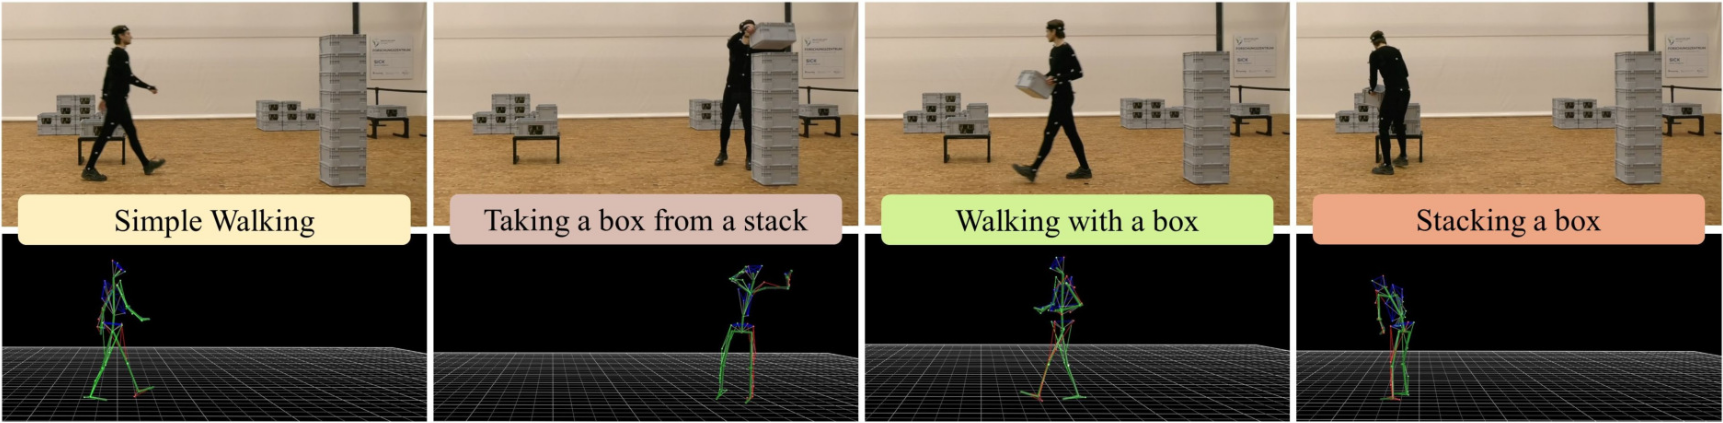
\includegraphics[width=\textwidth]{har-image-skeleton.png}
    \caption{Example of human activities in a warehouse context.}
    \source
  \end{figure}
  \begin{itemize}
      \item Motion capturing costly
      \item Pose estimators become better rapidly
      \item End-to-end training recently proposed
  \end{itemize}
  \footnotetext[1]{\cite{reining_towards_2018}}
\end{myframe}

\tableofcontents

\section{Fundamentals}
\subsection{Human Activity Recognition}

\begin{myframe}[Fundamentals - HAR]
    \note[item]{Human Action Recognition}
    \note[item]{Kontrolle von Mitarbeitern}
    \note[item]{Steuerung von Computern mit Gesten}
    \note[item]{Beispiele: Gehen, hinlegen, telefonieren etc.}
    \begin{columns}
        \begin{column}{.48\textwidth}
            \begin{itemize}
                \item Identify actions performed by humans
                \item Some use-cases:
                    \begin{itemize}
                        \item Video surveillance
                        \item Human-computer interaction
                        \item Computer animation
                        \item Warehouse scenario from before
                    \end{itemize}
                \item Multiple sources for detection
                \begin{itemize}
                    \item Inertial Measurement Units (IMUs)
                    \item Images (or \textbf{video})
                \end{itemize}
            \end{itemize}
        \end{column}
        \begin{column}{.48\textwidth}
            \begin{figure}
                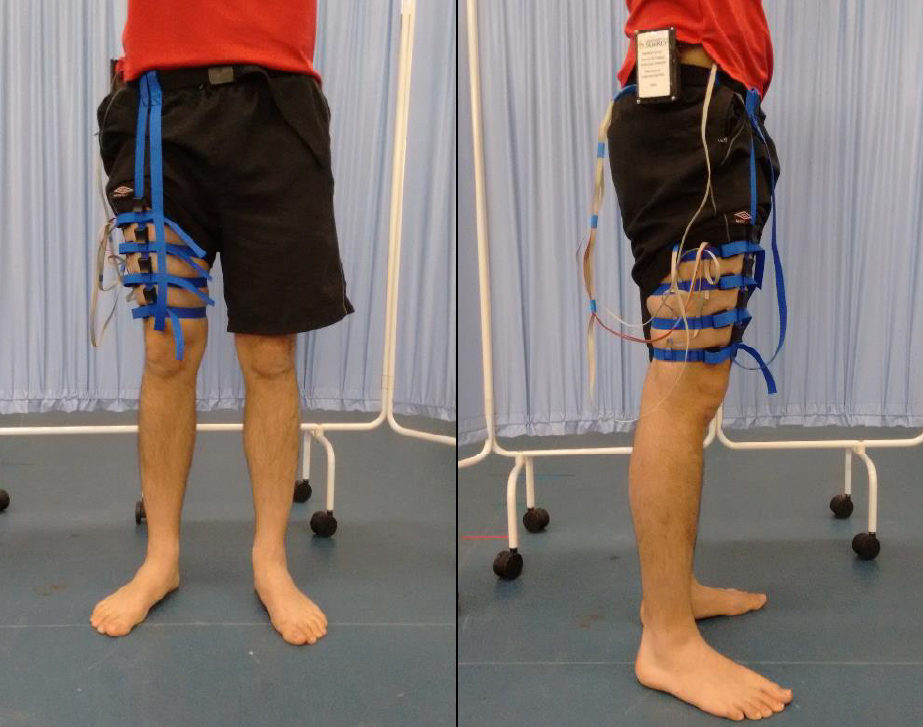
\includegraphics[width=0.99\textwidth]{imu.jpg}
                \caption{Inertial Measurement Units manufactured by Surrey Sensors}
                \source
            \end{figure}
        \end{column}
    \end{columns}
    \footnotetext[1]{\url{http://surreysensors.com/wp-content/uploads/2017/02/IMU.jpg}}
\end{myframe}

\begin{myframe}[Fundamentals - HAR]
    \note[item]{Menschliche Handlungen sind stark unterschiedlich da auch Menschen stark unterschiedlich sind (Kleidung, Körperform etc.)}
    \note[item]{Dicke Winterjacke vs. nur Unterhemd}
    \note[item]{}
    \note[item]{Action aus Attributen zusammengesetzt}
    \begin{columns}
        \begin{column}{.48\linewidth}
            \begin{itemize}
                \item \textbf{Some challenges:}
                    \begin{itemize}
                        \item High degree of interclass variance
                        \item How fine-grained?
                        \begin{itemize}
                            \item \textit{Raising left arm} or
                            \item \textit{Waving}
                            \item \textit{attributes} vs. \textit{actions} \footnotemark
                        \end{itemize}
                    \end{itemize}
            \end{itemize}
        \end{column}
        \begin{column}{.48\linewidth}
            \begin{figure}
                \includegraphics[width=0.99\textwidth]{attributes-actions.png}
                \sourcefix{1}
            \end{figure}
        \end{column}
    \end{columns}
    \footnotetext[1]{\cite{reining_towards_2018}}
\end{myframe}

\subsection{Pose Estimation}

\begin{myframe}[Fundamentals - Pose Estimation]
    \note[item]{Extrahierung von Gelenkpunkten aus Bild (Heatmap oder Regression, je nach Anstatz)}
    \note[item]{Es gibt verschiedene Ansätze und Anzahl an Punkten. Manchmal Gesicht in verschiedene Punkte unterteilt}
    \begin{columns}[T]
        \begin{column}{0.45\textwidth}
            \vspace{30px}
            \begin{itemize}
                \item Detect joint locations
                \item Different definitions
                \item Single vs. multi person
            \end{itemize}
        \end{column}
        \begin{column}{0.55\textwidth}
            \begin{figure}
                \includegraphics[width=.89\textwidth]{pe-singlehumna.png}
                \source
            \end{figure}
        \end{column}
    \end{columns}
    \begin{figure}
        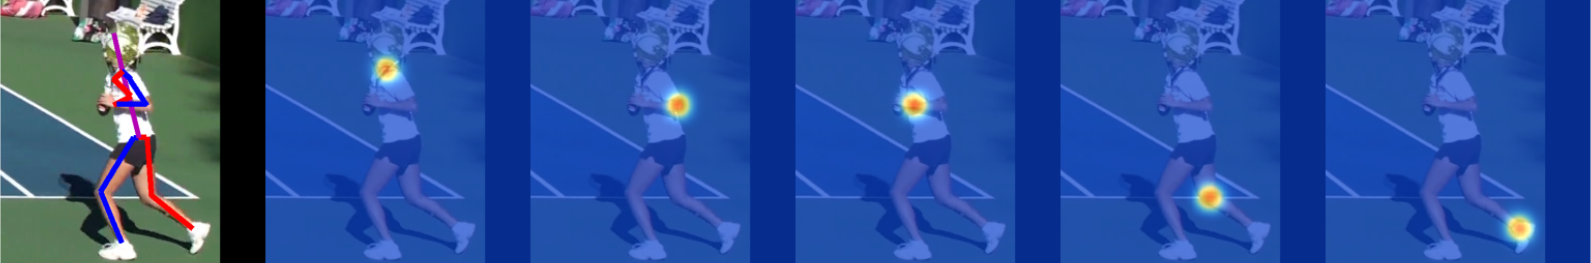
\includegraphics[height=50px]{2dheatmaps.png}
        \source
    \end{figure}
    \footnotetext[1]{\url{https://blog.nanonets.com/content/images/2019/04/Screen-Shot-2019-04-11-at-5.17.56-PM.png}}
    \footnotetext[2]{\cite{newell_stacked_2016}}
\end{myframe}

\begin{myframe}[Fundamentals - Pose Estimation]
    \note[item]{\textbf{Probleme}: Überlappung und Verdeckung , nicht nur bei mehreren Personen pro Bild}
    \begin{figure}
        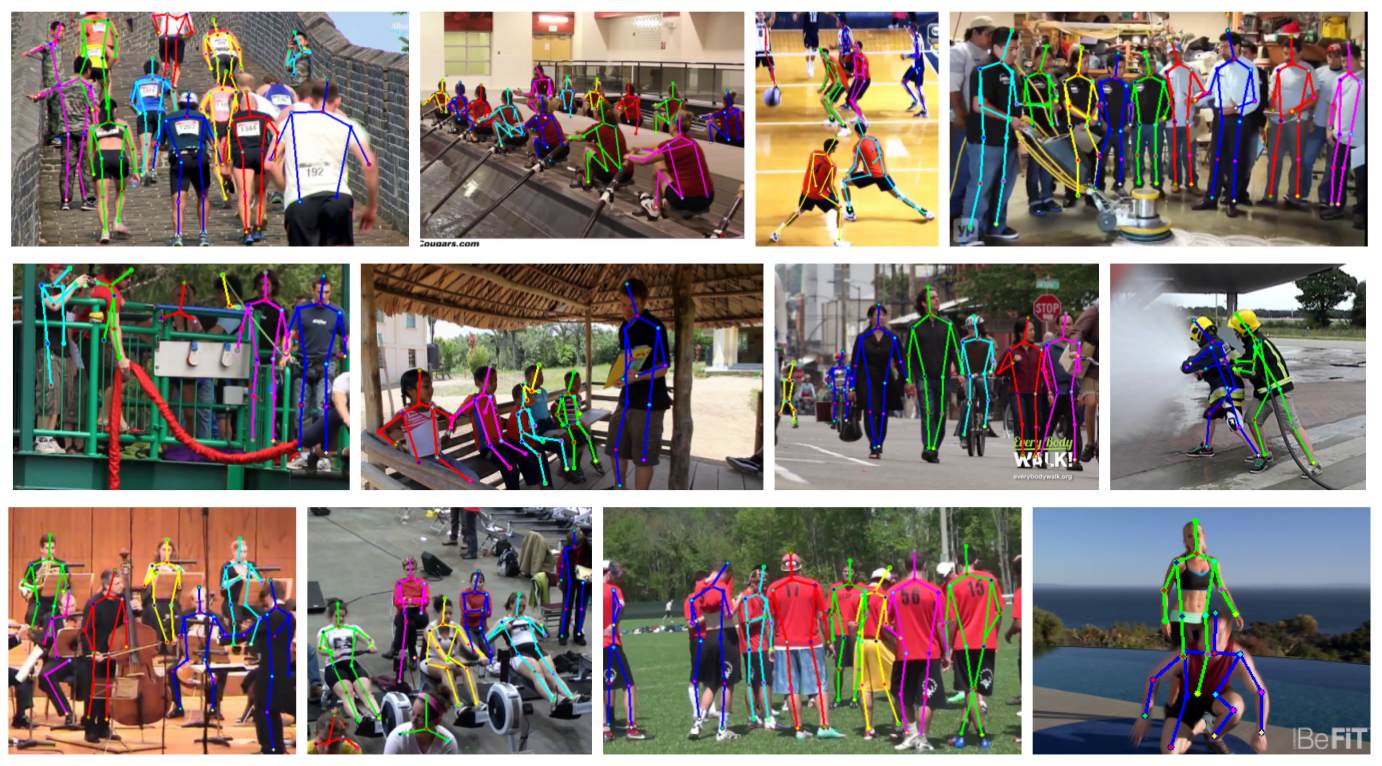
\includegraphics[width=.99\textwidth]{pe-multihuman.png}
        \caption{Example of hard multi-person pose estimation situations.}
        \source
    \end{figure}
    \footnotetext[1]{\url{http://pages.iai.uni-bonn.de/iqbal_umar/multiperson-pose/}}
\end{myframe}

\section{Related Work}
\subsection{Pose Estimation}

\begin{myframe}[Pose Estimation - Shallow Methods]
    \note[item]{Ansatz: Menschliches Skelet besteht aus Strukturen (Gliedmaßen) welche mit "Federn" verbunden sind. (\textit{also keine Gelenkpunkte})}
    \note[item]{$c$: Parameter welche gelernt werden. Sie geben an, wie die Gaussparameter sind etc.}
    \note[item]{Chamfer Distanz gibt an wie gut matching ist}
    \note[item]{}
    \note[item]{Approximate each limb as rectangle using $\ell = (x,y,s,\theta)$}
    \note[item]{Maximize covered foreground pixels by parts $p(I \lvert \ell,c)$}
    \note[item]{Relative positions / rotations between limbs $p(\ell_i,\ell_j \lvert c_{ij})$}
    \begin{columns}[T]
        \begin{column}{.48\textwidth}
            \begin{itemize}
                \item \textbf{Pictoral Structures for Object Recognition \footnotemark}
              \begin{itemize}
                  \item Based on initial work by \footnotemark
                  \item Binary images (background subtraction)
                  \item \textit{Model each limb}
                  \begin{itemize}
                      \item Approximate each limb as rectangle
                      \item Maximize covered foreground pixels by parts
                  \end{itemize}
                  \item \textit{Relation between limbs}
                  \begin{itemize}
                      \item Relative positions / rotations between limbs
                  \end{itemize}
                  \item Maximum likelihood estimation
                  \item Chamfer Distance to evaluate sampled configurations
              \end{itemize}
            \end{itemize}
        \end{column}
        \footnotetext[1]{\cite{felzenszwalb_pictorial_2005}}
        \footnotetext[2]{\cite{fischler_representation_1973}}
        \begin{column}{.48\textwidth}
            \begin{figure}
                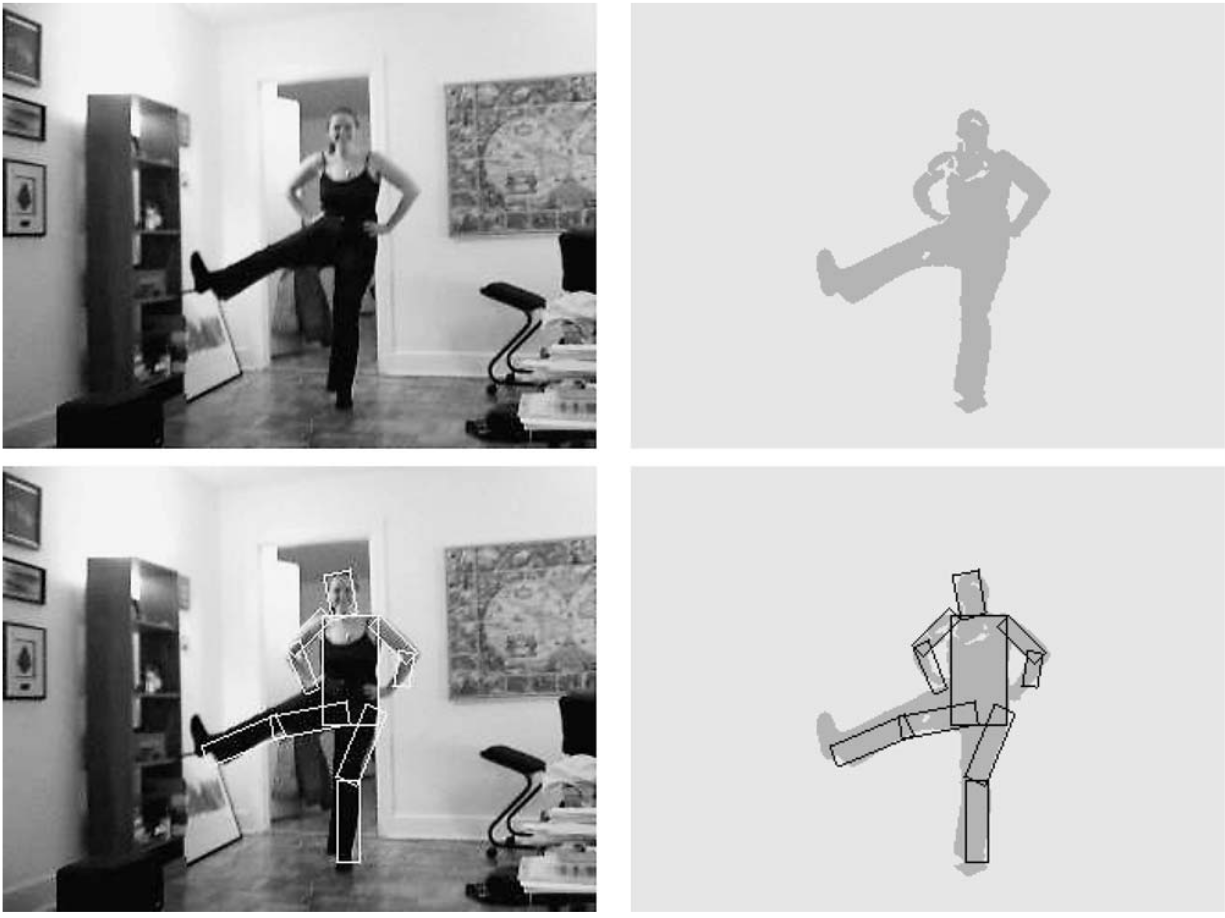
\includegraphics[width=.99\textwidth]{felzenszwalb-overview.png}
                \sourcefix{1}
            \end{figure}
        \end{column}
    \end{columns}
\end{myframe}

\begin{myframe}[Pose Estimation - Deep Methods]
    \note[item]{Netz basiert vollständig aus Faltungsschichten (fully convolutional)}
    \note[item]{Durch Pooling Auflösung verringern und durch Upsampling wiederherstellen.}
    \note[item]{Features aus den Zwischenschritten über Skip-connections weiterverwenden}
    \note[item]{Wichtig für Kombination von Features auf verschiedenen skalierungsstufen}
    \note[item]{}
    \note[item]{Durch aufeinanderfolgen: Initiale Ergebnisse werden immer weiter verfeinert und verbessert}
    \begin{columns}[T]
        \begin{column}{.48\textwidth}
            \begin{itemize}
                \item \textbf{Stacked hourglass network \footnotemark}
                  \begin{itemize}
                    \item \textbf{Hourglass}
                    \begin{itemize}
                        \item Pooling, upsampling, skip-connections
                        \item Intermediate supervision
                    \end{itemize}
                    \item \textbf{Stacked architectures}
                    \begin{itemize}
                        \item 8 hourglasses back-to-back
                        \item Refine result with each hourglass
                    \end{itemize}
                  \end{itemize}
            \end{itemize}
        \end{column}
        \footnotetext[1]{\cite{newell_stacked_2016}}
        \begin{column}{.48\textwidth}
            \begin{figure}
                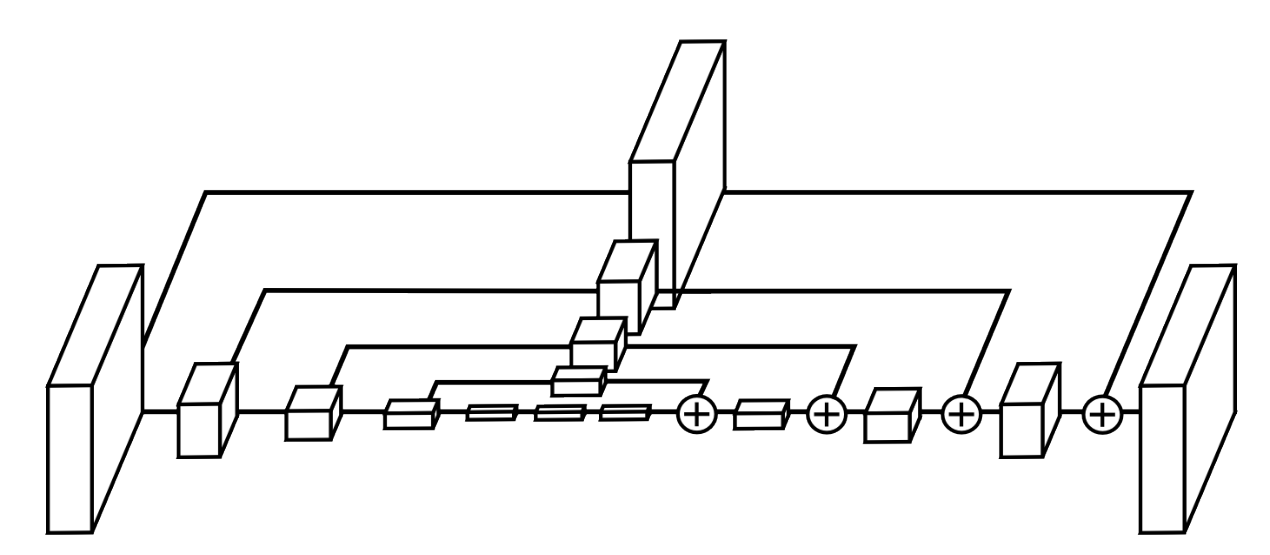
\includegraphics[width=.65\textwidth]{single-hourglass.png}
                \sourcefix{1}
            \end{figure}
        \end{column}
    \end{columns}
    \begin{figure}
        \includegraphics[width=.65\textwidth]{stackedhourglass.png}
        \sourcefix{1}
    \end{figure}
\end{myframe}

\begin{myframe}[Stacking architectures - Qualitative evaluations]
    \note[item]{Verfeinern der initialen Vorhersage und korrigieren von Fehlern z.B. Rechte Hand von anderer Person im Bild fälschlicherweise erkannt}
    \note[item]{Dadurch, dass spätere Module die Informationen von vorherigen bekommen können sie beispielsweise bei der Entscheidung "Welche Pixel gehöhren zum rechten Ellenbogen?" die vorherigen Ergebnisse für "Rechte Schulter" miteinbeziehen, welche in der Praxis oft einfacher zu finden sind.}
    \note[item]{Selbst wenn \textbf{noisy} trotzdem von Vorteil.}
    \begin{figure}
        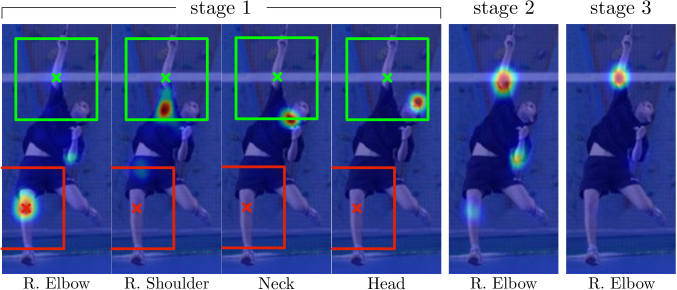
\includegraphics[width=0.75\textwidth]{context-belief-maps.png}
        \caption{Easier to detect features like head and neck can influence the detection of harder features like elbows and knees. Thus, an initially wrong result (see \textit{R. Elbow} in Stage 1) can be corrected in later stages.\fcite{newell_stacked_2016}}
    \end{figure}
    \begin{figure}
        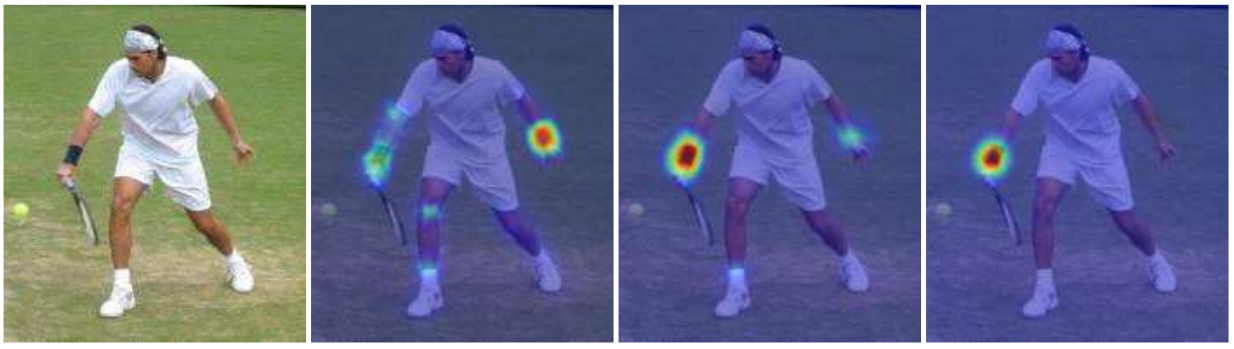
\includegraphics[width=0.55\textwidth]{cpm-qualitative.png}
        \caption{Another qualitative example of stacked architectures improving on intermediate results \fcite{wei_convolutional_2016}}
    \end{figure}
\end{myframe}

\subsection{Video-based HAR}

\begin{myframe}[Video-based HAR - Shallow Methods]
    \note[item]{Video als Würfel}
    \note[item]{Interest Points dort wo starke Veränderungen in $x$, $y$ und $t$ stattfinden}
    \note[item]{Cluster mittels k-means, $k = 4000$, aus Trainingsdaten}
	\begin{itemize}
		\item \textbf{Learning Realistic Human Actions from Movies \fcite{laptev_learning_2008}}
		\begin{itemize}
			\item Spatio-temporal extension of Harris corner detection
			\item Volume around interest points
			\begin{itemize}
                \item \textit{Histogram of oriented gradients (HoG)}
                \item \textit{Histogram of optical flow (HoF)}
				\item concatenation and normalization
			\end{itemize}
			\item Clustering into Bag-of-features
            \item Classification using Support Vector Machines (SVM)
		\end{itemize}
	\end{itemize}
	\begin{figure}
		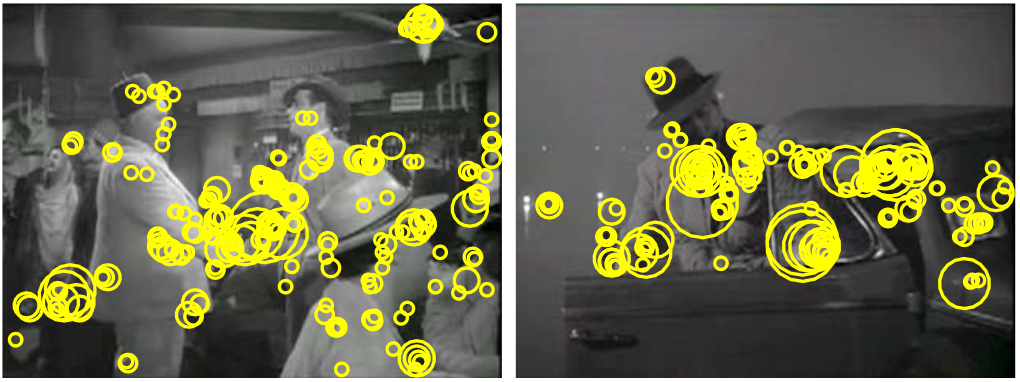
\includegraphics[width=.7\textwidth]{spacetimeinterestpoints.png}
        \caption{Left: Shaking hand, right: getting out of car.}
        \sourcefix{1}
	\end{figure}
\end{myframe}

\begin{myframe}[Video-based HAR - Deep Methods]
    \note[item]{Dritte Dimension $\Rightarrow$ Zeit}
    \note[item]{3D convolutions sind schwer dafür geeignet tiefe netze zu bilden da sie sehr viele parameter haben.}
    \note[item]{Darum werden auch sehr sehr sehr große Datensets benötigt weil schwerer zu lernen.}
    \note[item]{Kurz: Geht nicht tief genug weil zu viele Ressourcen benötigt würden.}
    \note[item]{Darum: Kombination aus tiefen 2D und 3D}
    \note[item]{Zwei Ansätze zur Kombination:}
    \note[item]{\textbf{Konkatenation}: 3D Convolution auf Input und dann auf die 2D output feature map nochmal 2D Convolution}
    \note[item]{\textbf{Addition}: Output der 3D convolution wird addiert mit dem output einer 2D convolution auf dem letzten Frame.}
    \note[item]{Kombination von beiden findet statt (siehe figure)}

	\begin{itemize}
		\item \textbf{MiCT: Mixed Convolutional Tube \fcite{zhou_mict:_2018}}
		\begin{itemize}
			\item Third dimension $\Rightarrow$ temporal dimension
			\item Combining 2D and 3D convolutions more accurate than just 3D
			\item 4 MiCT blocks, followed by fully-connected layer
			\item State-of-the-art on HMDB51 for RGB-only methods
		\end{itemize}
	\end{itemize}
	\begin{figure}
		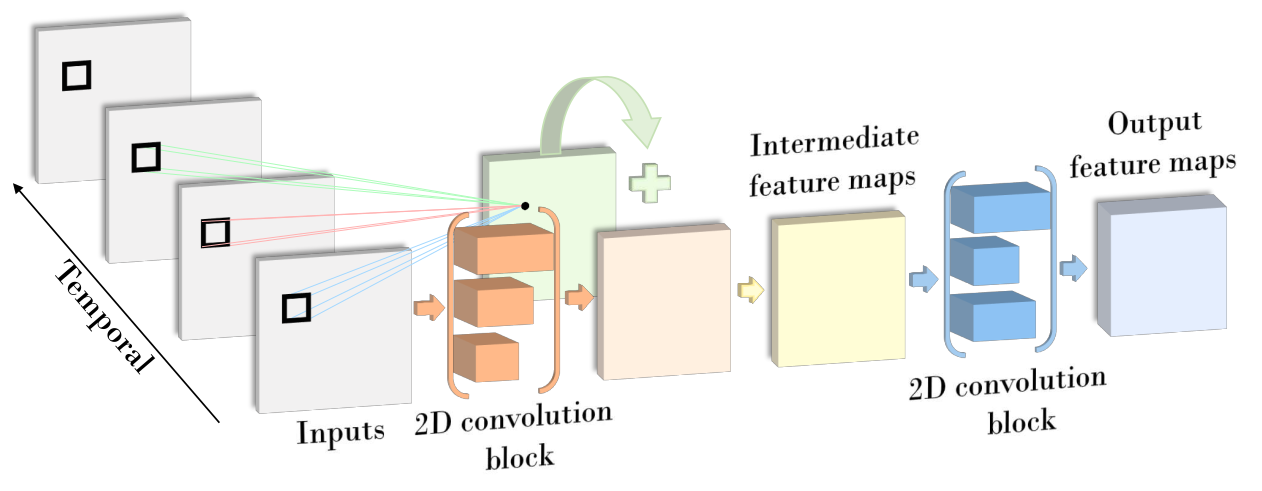
\includegraphics[width=.7\textwidth]{mict-block.png}
        \caption{Combining simple 2D convolutions with 3D convolutions.}
        \sourcefix{1}
	\end{figure}
\end{myframe}

\section{Method}

\begin{myframe}[Method - Joint methods]
    \note[item]{Handlungserkennung und Posenbestimmung gemeinsam trainieren. Idee: Profitieren voneinander}
    \note[item]{ Pretraining von Pose (Verschiedene Datensätze für Pose und Action)}
    \note[item]{Optimierung (fine-tuning) passiert end-to-end}
    \note[item]{}
    \note[item]{Oft ist die Ausgabe von neuronalen Netzen zur Posenbestimmung eine Heatmap. Heatmap stellt Softmaxverteilung da}
    \note[item]{\textbf{Argmax als postprocessing schritt nötig} damit exakte Koordinaten. Wenn man end-to-end trainieren will ist ein nicht-differentierbares Argmax aber problematisch.}
    \note[item]{Normalisierte Version des Erwartungswerts des Softmax in x und y Dimension}
	\begin{columns}[T]
	\begin{column}{.45\textwidth}
		\begin{itemize}
			\item \textbf{Multitask Deep HAR}\footnotemark
			\begin{itemize}
                \item Jointly train pose and action recognition
                \item Pre-train pose estimation part, then fine-tune end-to-end
				\item \textit{Soft-argmax}\footnotemark~makes end-to-end learning possible
			\end{itemize}
		\end{itemize}
        \begin{figure}
            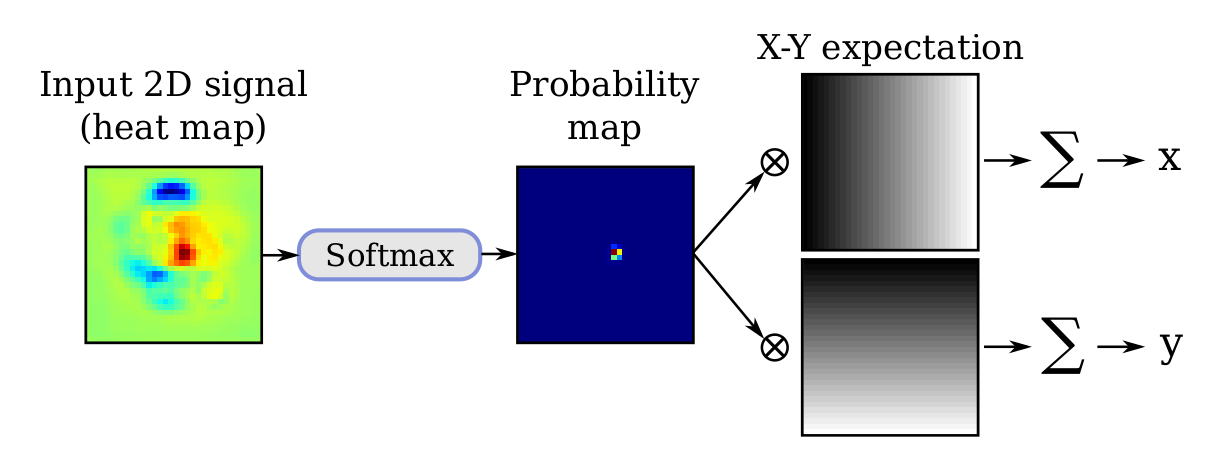
\includegraphics[width=0.99\textwidth]{softargmax.png}
            \sourcefix{1}
        \end{figure}
	\end{column}
    \footnotetext[1]{\cite{luvizon_2d/3d_2018}}
    \footnotetext[2]{\cite{luvizon_human_2017}}
	\begin{column}{.45\textwidth}
		\begin{figure}
			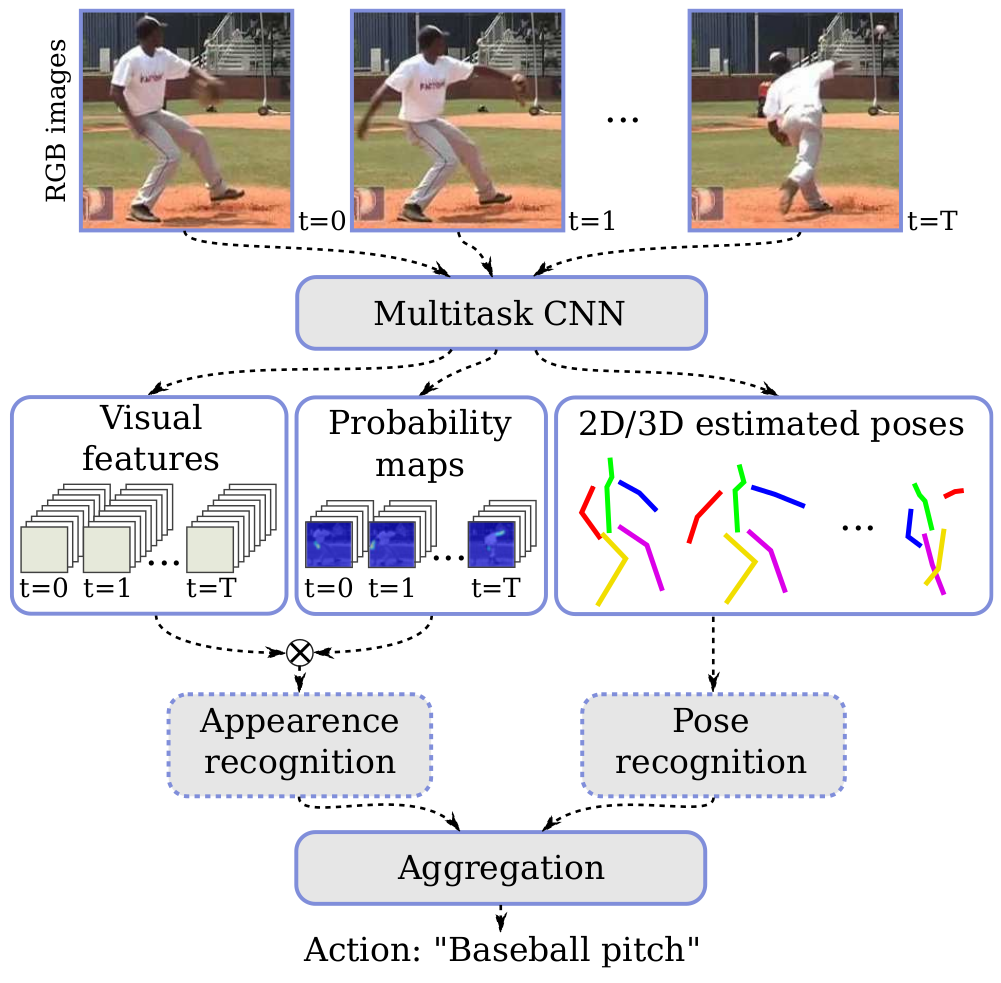
\includegraphics[width=.99\textwidth]{endtoend-concept.png}
            \sourcefix{1}
            %\caption{Complete network pipeline.}
		\end{figure}
	\end{column}
	\end{columns}
\end{myframe}

\begin{myframe}[Multitask Deep HAR - Architecture]
    \note[item]{Basiert auf Inception v4 um Features zu extrahieren}
    \note[item]{Prediction Blocks: Ähnlich zu Hourglasses von vorhin. Nach jedem Block ein Zwischenergebnis welches verfeinert wird.}
    \note[item]{Nach \textbf{jedem} prediction block: Heatmap (Softargmax) und Wahrscheinlichkeitsvektor}
    \note[item]{Loss: Elstic Net loss}


    \begin{columns}[T]
        \begin{column}{.45\textwidth}
            \begin{itemize}
                \item \textit{Multitask CNN}
                \begin{itemize}
                    \item Blocks similar to hourglasses
                    \item Refine prediction with each additional block
                    \item In addition to providing visual features and heatmaps:
                    \begin{itemize}
                        \item Coordinates from Soft-argmax
                        \item Join visibility vector using sigmoid
                    \end{itemize}
                    \item Loss function $$L_p = \frac{1}{N_J}\sum_{n=1}^{N_J}(~ \lvert\lvert \hat{p}_n - p_n \rvert\rvert_1 ~+~ \lvert\lvert \hat{p}_n - p_n \rvert\rvert^2_2 ~ )$$
                \end{itemize}
            \end{itemize}
        \end{column}
        \begin{column}{.45\textwidth}
            \begin{figure}
                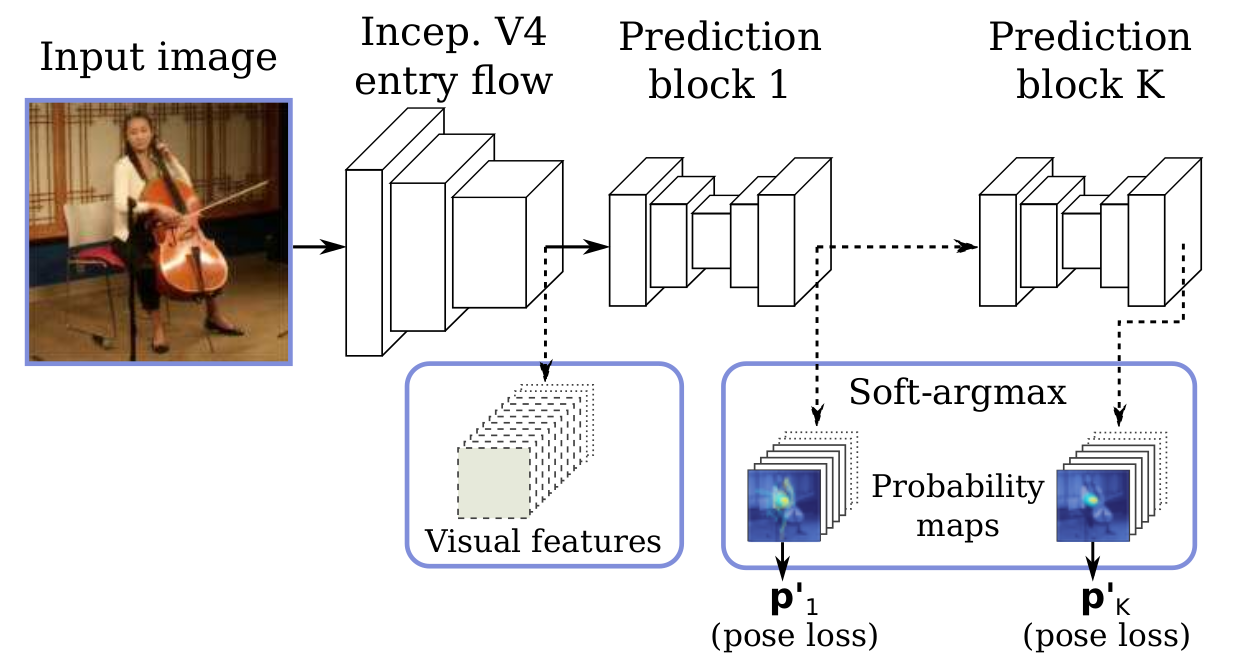
\includegraphics[width=.99\textwidth]{multitask-part.png}
                \sourcefix{1}
            \end{figure}
        \end{column}
	\end{columns}
    \footnotetext[1]{\cite{luvizon_2d/3d_2018}}
\end{myframe}

\begin{myframe}[Multitask Deep HAR - Architecture]
    \note[item]{Pipeline zu sehen.}
    \note[item]{Auch hier: keine genauen Angaben zum Aufbau. Verweis auf Code}
    \note[item]{Action Heatmap für jede Handlung. Mittles Pooling und Softmax dann Wahrscheinlichkeit}
    \note[item]{Max+Min pooling: $f(x) = \text{MaxPooling}(x) - \text{MaxPooling}(-x)$}

	\begin{columns}[T]
        \begin{column}{.45\textwidth}
            \begin{itemize}
                \item \textit{Pose recognition}
                \begin{itemize}
                    \item Arrange joint values over time in 2D matrix
                    \item Action heatmaps
                    \begin{itemize}
                        \item Through softmax: action probabilities
                    \end{itemize}

                \end{itemize}
            \end{itemize}
        \end{column}
        \begin{column}{.45\textwidth}
            \begin{figure}
                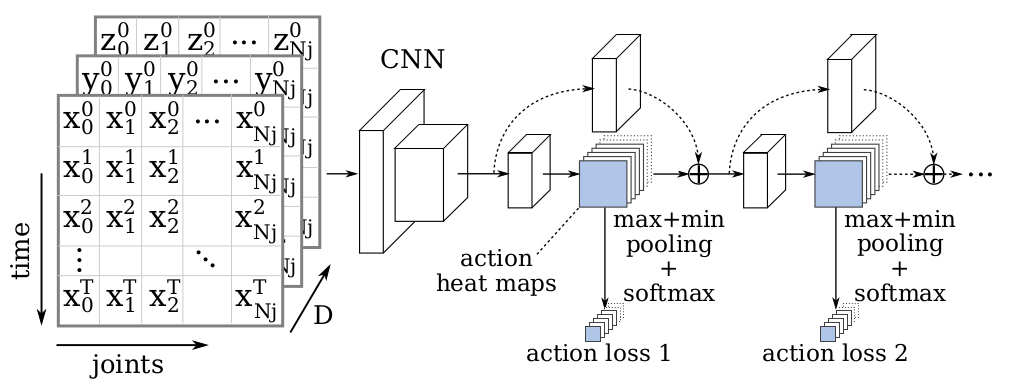
\includegraphics[width=.99\textwidth]{jointsovertime.png}
                \sourcefix{1}
            \end{figure}
        \end{column}
	\end{columns}
    \footnotetext[1]{\cite{luvizon_2d/3d_2018}}
\end{myframe}

\begin{myframe}[Multitask Deep HAR - Architecture]
    \note[item]{Im Prinzip gleicher Aufbau wie vorher, nur mit Visual Features statt Posen}
    \note[item]{\textbf{Am Ende:}}
    \note[item]{Durch FC-Layer aggregation und mit softmax dann finales Ergebnis}
	\begin{columns}[T]
        \begin{column}{.45\textwidth}
            \begin{itemize}
                \item \textit{Appearance recognition}
                \begin{itemize}
                    \item Combination of visual features and joint positions
                    \item Then: Identical architecture to pose recognition part
                \end{itemize}
                \item \textit{Aggregation}
                \begin{itemize}
                    \item Combine pose recognition and appearance recognition for final result
                    \item \textit{Categorical cross-entropy}
                \end{itemize}
            \end{itemize}
        \end{column}
        \begin{column}{.45\textwidth}
            \begin{figure}
                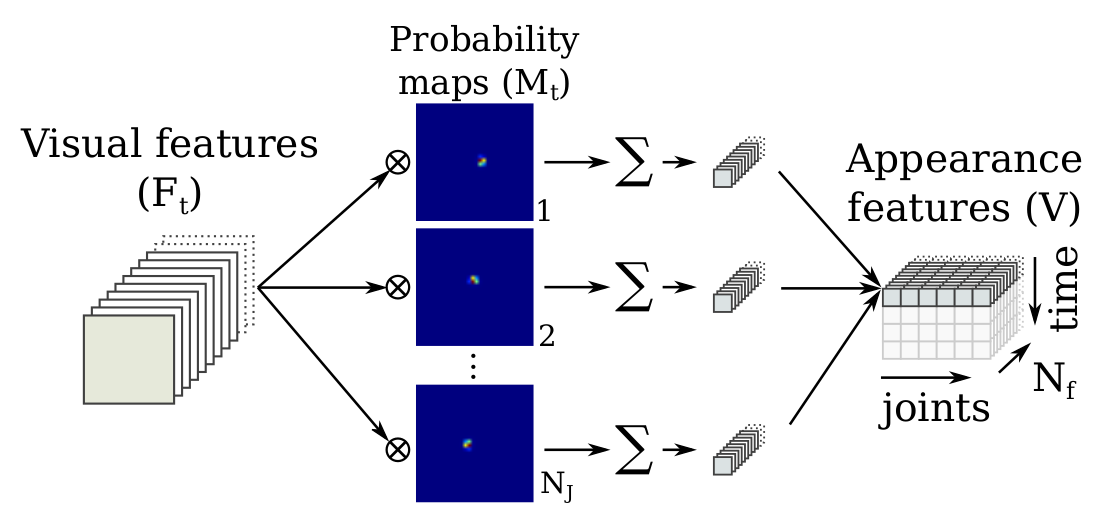
\includegraphics[width=.99\textwidth]{appearance-features.png}
                \sourcefix{1}
            \end{figure}
        \end{column}
	\end{columns}
    \footnotetext[1]{\cite{luvizon_2d/3d_2018}}
\end{myframe}

\begin{myframe}[Method]
    \begin{itemize}
        \item Reimplementation in PyTorch \fcite{paszke_automatic_2017}
        \begin{itemize}
            \item Evaluate against HMDB \fcite{kuehne_hmdb:_2011}
        \end{itemize}
        \item Experimentation
        \begin{itemize}
            %\item Better incorporation of temporal dimension \fcite{pavllo_3d_2019}
            \item Compare with state-of-the-art methods not using pose \fcite{zhou_mict:_2018}
            \item Different representation of temporal information (next slide)
            \item Combined loss function of pose and action for \emph{real} end-to-end training
        \end{itemize}
    \end{itemize}
\end{myframe}

\begin{myframe}[Method]
    \note[item]{Dadurch: Eine Repräsentation für Video features und IMU Datenströme. \textit{Kombination?}}
    \begin{figure}
        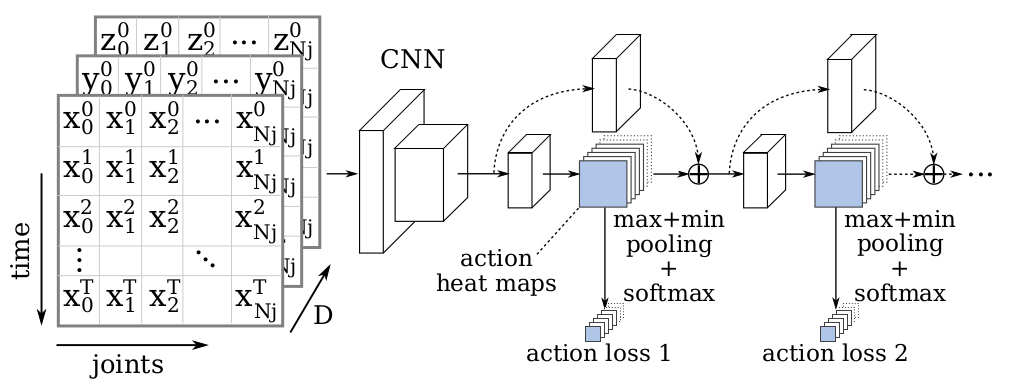
\includegraphics[width=.65\textwidth]{jointsovertime.png}
        \caption{Approach used by \footnotemark. Convolution over all sensors at once. \sourcefix{1}}
    \end{figure}
    \begin{figure}
        \includegraphics[width=.65\textwidth]{sensor-time.png}
        \caption{Impression of pixel coordinates of joints over time \source}
    \end{figure}
    \footnotetext[1]{\cite{luvizon_2d/3d_2018}}
    \footnotetext[2]{\url{https://avtech.com/articles/wp-content/uploads/2015/06/Intro.-Pic.png}}
\end{myframe}

\section{Datasets}
% also: metrics?
% \begin{myframe}[2D / 3D pose datasets]
%   \begin{itemize}
%       \item \textbf{2D}
%       \begin{itemize}
%           \item MPII \fcite{andriluka_2d_2014}
%           \item LSP \fcite{johnson_clustered_2010}\fcite{johnson_learning_2011}
%       \end{itemize}
%       \item \textbf{3D}
%       \begin{itemize}
%           \item Human 3.6M \fcite{ionescu_human3.6m:_2014}
%       \end{itemize}
%   \end{itemize}
% \end{myframe}

\begin{myframe}[2D Pose Datasets]
  \begin{columns}[T]
      \begin{column}{.48\textwidth}
          \begin{itemize}
              \item \textbf{MPII Human Pose\footnotemark}
              \begin{itemize}
                  \item 40,000 annotated images
                  \item Single and multi person
                  \item Over 401 different activities
              \end{itemize}
          \end{itemize}
      \end{column}
      \footnotetext[1]{\cite{andriluka_2d_2014}}
      \begin{column}{.48\textwidth}
          \begin{figure}
              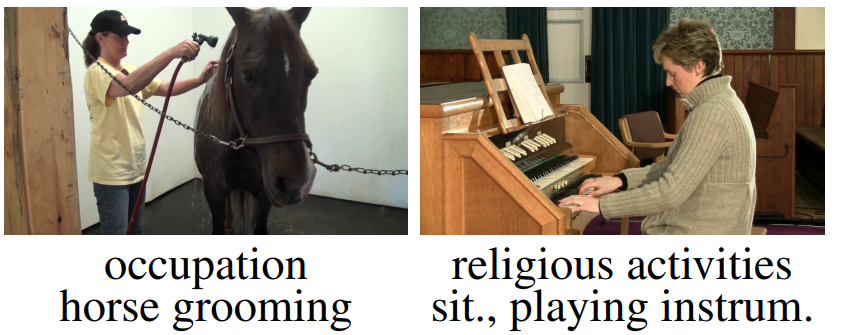
\includegraphics[width=0.99\textwidth]{mpii.png}
              \sourcefix{1}
          \end{figure}
      \end{column}
  \end{columns}
\end{myframe}

% \begin{myframe}[3D Pose Datasets]
%   \begin{columns}[T]
%       \begin{column}{.48\textwidth}
%           \vspace{50px}
%           \begin{itemize}
%               \item \textbf{Human3.6m\footnotemark}
%               \begin{itemize}
%                   \item 3,600,000 annotated images
%                   \item Annotated using motion capturing system
%                   \item 11 male and female actors recreate daily situations
%                   \item 17 different scenarios
%               \end{itemize}
%           \end{itemize}
%       \end{column}
%       \footnotetext[1]{\cite{ionescu_human3.6m:_2014}}
%       \begin{column}{.48\textwidth}
%           \begin{figure}
%               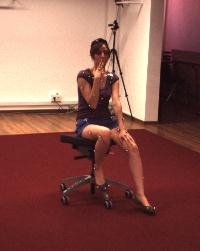
\includegraphics[width=0.48\textwidth]{human-01.jpg}
%               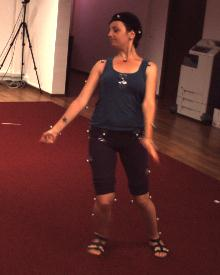
\includegraphics[width=0.48\textwidth]{human-02.jpg}
%               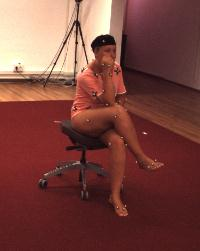
\includegraphics[width=0.48\textwidth]{human-03.jpg}
%               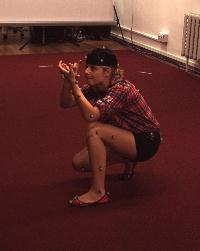
\includegraphics[width=0.48\textwidth]{human-04.jpg}
%               \source
%           \end{figure}
%       \end{column}
%   \end{columns}
%   \footnotetext[2]{\url{http://vision.imar.ro/human3.6m/description.php}}
% \end{myframe}

% \begin{myframe}[2D HAR datasets]
%   \begin{itemize}
%       \item Penn Action \fcite{zhang_actemes_2013}
%       \item HMDB51 \fcite{kuehne_hmdb:_2011}
%       \item Kinetics \fcite{kay_kinetics_2017}
%   \end{itemize}
% \end{myframe}

\begin{myframe}[Action Recognition Datasets]
  \begin{columns}[T]
      \begin{column}{.48\textwidth}
          \vspace{20px}
          \begin{itemize}
              \item \textbf{Penn Action\footnotemark}
              \begin{itemize}
                  \item 2,400 video clips of 15 actions
                  \item Very limited number of actions (mainly sport)
              \end{itemize}
          \end{itemize}
      \end{column}
      \footnotetext[1]{\cite{zhang_actemes_2013}}
      \begin{column}{.48\textwidth}
          \begin{figure}
              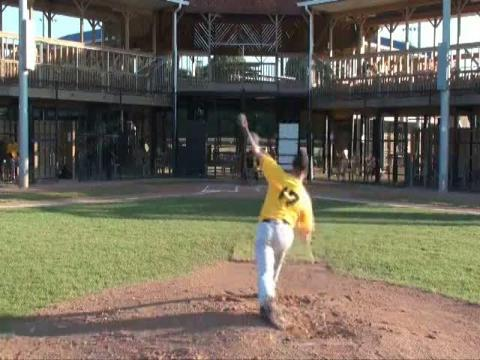
\includegraphics[height=45px]{pa-01.jpg}
              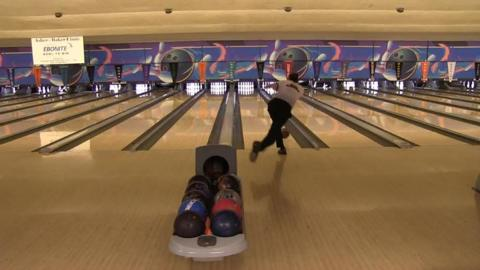
\includegraphics[height=45px]{pa-02.jpg}
              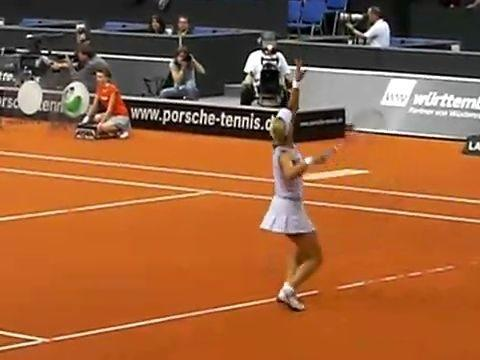
\includegraphics[height=45px]{pa-03.jpg}
              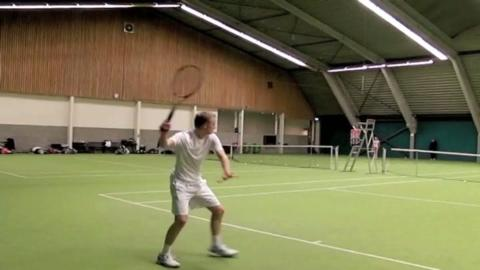
\includegraphics[height=45px]{pa-04.jpg}
              \source
          \end{figure}
      \end{column}
  \end{columns}
  \footnotetext[2]{\url{https://upenn.app.box.com/v/PennAction}}
\end{myframe}

\begin{myframe}[Action Recognition Datasets]
  \begin{columns}[T]
      \begin{column}{.48\textwidth}
          \begin{itemize}
              \item \textbf{HMDB51\footnotemark}
              \begin{itemize}
                  \item 6,800 video clips of 51 actions
                  \item Video clips from Youtube
                  \item At least 101 clips per action category
              \end{itemize}
          \end{itemize}
      \end{column}
      \footnotetext[1]{\cite{kuehne_hmdb:_2011}}
      \begin{column}{.48\textwidth}
          \begin{figure}
              \includegraphics[height=.55\textheight]{hmdb-example.png}
              \source
          \end{figure}
      \end{column}
  \end{columns}
  \footnotetext[2]{\url{http://serre-lab.clps.brown.edu/wp-content/uploads/2012/08/HMDB_snapshot1.png}}
\end{myframe}

\begin{myframe}[Action Recognition Datasets]
  \begin{columns}[T]
      \begin{column}{.48\textwidth}
          \begin{itemize}
              \item \textbf{J-HMDB\footnotemark}
              \begin{itemize}
                  \item Fully-annotated subset of HMDB
                  \begin{itemize}
                      \item 2D pose, person segmentation maps etc.
                  \end{itemize}
                  \item 928 clips of 21 actions
                  \item Can be used for end-to-end training
              \end{itemize}
          \end{itemize}
      \end{column}
      \footnotetext[1]{\cite{jhuang_towards_2013}}
      \begin{column}{.48\textwidth}
          \begin{figure}
              \includegraphics[height=.55\textheight]{jhmdb.png}
              \centering
              \source
          \end{figure}
      \end{column}
  \end{columns}
  \footnotetext[2]{\url{http://jhmdb.is.tue.mpg.de/puppet_tool}}
\end{myframe}

\section{Conclusion}
\begin{myframe}[Conclusion]
    \begin{itemize}
        \item Promising results combining pose and action recognition
        \item But: Barely any publications in the past year
        \item Much experimentation possible
        \item Future work:
        \begin{itemize}
            \item Multi-person end-to-end pipeline
            \item Bigger pose-annotated \emph{in-the-wild} action datasets necessary
        \end{itemize}
    \end{itemize}
\end{myframe}

\begin{myframe}[Thank you]
    \centering \Large
    \emph{Thank you for your time!}
\end{myframe}

\end{document}

